% Options for packages loaded elsewhere
\PassOptionsToPackage{unicode}{hyperref}
\PassOptionsToPackage{hyphens}{url}
\PassOptionsToPackage{dvipsnames,svgnames,x11names}{xcolor}
%
\documentclass[
  letterpaper,
  DIV=11,
  numbers=noendperiod]{scrartcl}

\usepackage{amsmath,amssymb}
\usepackage{iftex}
\ifPDFTeX
  \usepackage[T1]{fontenc}
  \usepackage[utf8]{inputenc}
  \usepackage{textcomp} % provide euro and other symbols
\else % if luatex or xetex
  \usepackage{unicode-math}
  \defaultfontfeatures{Scale=MatchLowercase}
  \defaultfontfeatures[\rmfamily]{Ligatures=TeX,Scale=1}
\fi
\usepackage{lmodern}
\ifPDFTeX\else  
    % xetex/luatex font selection
\fi
% Use upquote if available, for straight quotes in verbatim environments
\IfFileExists{upquote.sty}{\usepackage{upquote}}{}
\IfFileExists{microtype.sty}{% use microtype if available
  \usepackage[]{microtype}
  \UseMicrotypeSet[protrusion]{basicmath} % disable protrusion for tt fonts
}{}
\makeatletter
\@ifundefined{KOMAClassName}{% if non-KOMA class
  \IfFileExists{parskip.sty}{%
    \usepackage{parskip}
  }{% else
    \setlength{\parindent}{0pt}
    \setlength{\parskip}{6pt plus 2pt minus 1pt}}
}{% if KOMA class
  \KOMAoptions{parskip=half}}
\makeatother
\usepackage{xcolor}
\setlength{\emergencystretch}{3em} % prevent overfull lines
\setcounter{secnumdepth}{-\maxdimen} % remove section numbering
% Make \paragraph and \subparagraph free-standing
\ifx\paragraph\undefined\else
  \let\oldparagraph\paragraph
  \renewcommand{\paragraph}[1]{\oldparagraph{#1}\mbox{}}
\fi
\ifx\subparagraph\undefined\else
  \let\oldsubparagraph\subparagraph
  \renewcommand{\subparagraph}[1]{\oldsubparagraph{#1}\mbox{}}
\fi

\usepackage{color}
\usepackage{fancyvrb}
\newcommand{\VerbBar}{|}
\newcommand{\VERB}{\Verb[commandchars=\\\{\}]}
\DefineVerbatimEnvironment{Highlighting}{Verbatim}{commandchars=\\\{\}}
% Add ',fontsize=\small' for more characters per line
\usepackage{framed}
\definecolor{shadecolor}{RGB}{241,243,245}
\newenvironment{Shaded}{\begin{snugshade}}{\end{snugshade}}
\newcommand{\AlertTok}[1]{\textcolor[rgb]{0.68,0.00,0.00}{#1}}
\newcommand{\AnnotationTok}[1]{\textcolor[rgb]{0.37,0.37,0.37}{#1}}
\newcommand{\AttributeTok}[1]{\textcolor[rgb]{0.40,0.45,0.13}{#1}}
\newcommand{\BaseNTok}[1]{\textcolor[rgb]{0.68,0.00,0.00}{#1}}
\newcommand{\BuiltInTok}[1]{\textcolor[rgb]{0.00,0.23,0.31}{#1}}
\newcommand{\CharTok}[1]{\textcolor[rgb]{0.13,0.47,0.30}{#1}}
\newcommand{\CommentTok}[1]{\textcolor[rgb]{0.37,0.37,0.37}{#1}}
\newcommand{\CommentVarTok}[1]{\textcolor[rgb]{0.37,0.37,0.37}{\textit{#1}}}
\newcommand{\ConstantTok}[1]{\textcolor[rgb]{0.56,0.35,0.01}{#1}}
\newcommand{\ControlFlowTok}[1]{\textcolor[rgb]{0.00,0.23,0.31}{#1}}
\newcommand{\DataTypeTok}[1]{\textcolor[rgb]{0.68,0.00,0.00}{#1}}
\newcommand{\DecValTok}[1]{\textcolor[rgb]{0.68,0.00,0.00}{#1}}
\newcommand{\DocumentationTok}[1]{\textcolor[rgb]{0.37,0.37,0.37}{\textit{#1}}}
\newcommand{\ErrorTok}[1]{\textcolor[rgb]{0.68,0.00,0.00}{#1}}
\newcommand{\ExtensionTok}[1]{\textcolor[rgb]{0.00,0.23,0.31}{#1}}
\newcommand{\FloatTok}[1]{\textcolor[rgb]{0.68,0.00,0.00}{#1}}
\newcommand{\FunctionTok}[1]{\textcolor[rgb]{0.28,0.35,0.67}{#1}}
\newcommand{\ImportTok}[1]{\textcolor[rgb]{0.00,0.46,0.62}{#1}}
\newcommand{\InformationTok}[1]{\textcolor[rgb]{0.37,0.37,0.37}{#1}}
\newcommand{\KeywordTok}[1]{\textcolor[rgb]{0.00,0.23,0.31}{#1}}
\newcommand{\NormalTok}[1]{\textcolor[rgb]{0.00,0.23,0.31}{#1}}
\newcommand{\OperatorTok}[1]{\textcolor[rgb]{0.37,0.37,0.37}{#1}}
\newcommand{\OtherTok}[1]{\textcolor[rgb]{0.00,0.23,0.31}{#1}}
\newcommand{\PreprocessorTok}[1]{\textcolor[rgb]{0.68,0.00,0.00}{#1}}
\newcommand{\RegionMarkerTok}[1]{\textcolor[rgb]{0.00,0.23,0.31}{#1}}
\newcommand{\SpecialCharTok}[1]{\textcolor[rgb]{0.37,0.37,0.37}{#1}}
\newcommand{\SpecialStringTok}[1]{\textcolor[rgb]{0.13,0.47,0.30}{#1}}
\newcommand{\StringTok}[1]{\textcolor[rgb]{0.13,0.47,0.30}{#1}}
\newcommand{\VariableTok}[1]{\textcolor[rgb]{0.07,0.07,0.07}{#1}}
\newcommand{\VerbatimStringTok}[1]{\textcolor[rgb]{0.13,0.47,0.30}{#1}}
\newcommand{\WarningTok}[1]{\textcolor[rgb]{0.37,0.37,0.37}{\textit{#1}}}

\providecommand{\tightlist}{%
  \setlength{\itemsep}{0pt}\setlength{\parskip}{0pt}}\usepackage{longtable,booktabs,array}
\usepackage{calc} % for calculating minipage widths
% Correct order of tables after \paragraph or \subparagraph
\usepackage{etoolbox}
\makeatletter
\patchcmd\longtable{\par}{\if@noskipsec\mbox{}\fi\par}{}{}
\makeatother
% Allow footnotes in longtable head/foot
\IfFileExists{footnotehyper.sty}{\usepackage{footnotehyper}}{\usepackage{footnote}}
\makesavenoteenv{longtable}
\usepackage{graphicx}
\makeatletter
\def\maxwidth{\ifdim\Gin@nat@width>\linewidth\linewidth\else\Gin@nat@width\fi}
\def\maxheight{\ifdim\Gin@nat@height>\textheight\textheight\else\Gin@nat@height\fi}
\makeatother
% Scale images if necessary, so that they will not overflow the page
% margins by default, and it is still possible to overwrite the defaults
% using explicit options in \includegraphics[width, height, ...]{}
\setkeys{Gin}{width=\maxwidth,height=\maxheight,keepaspectratio}
% Set default figure placement to htbp
\makeatletter
\def\fps@figure{htbp}
\makeatother

\usepackage{booktabs}
\usepackage{longtable}
\usepackage{array}
\usepackage{multirow}
\usepackage{wrapfig}
\usepackage{float}
\usepackage{colortbl}
\usepackage{pdflscape}
\usepackage{tabu}
\usepackage{threeparttable}
\usepackage{threeparttablex}
\usepackage[normalem]{ulem}
\usepackage{makecell}
\usepackage{xcolor}
\KOMAoption{captions}{tableheading}
\makeatletter
\makeatother
\makeatletter
\makeatother
\makeatletter
\@ifpackageloaded{caption}{}{\usepackage{caption}}
\AtBeginDocument{%
\ifdefined\contentsname
  \renewcommand*\contentsname{Table of contents}
\else
  \newcommand\contentsname{Table of contents}
\fi
\ifdefined\listfigurename
  \renewcommand*\listfigurename{List of Figures}
\else
  \newcommand\listfigurename{List of Figures}
\fi
\ifdefined\listtablename
  \renewcommand*\listtablename{List of Tables}
\else
  \newcommand\listtablename{List of Tables}
\fi
\ifdefined\figurename
  \renewcommand*\figurename{Figure}
\else
  \newcommand\figurename{Figure}
\fi
\ifdefined\tablename
  \renewcommand*\tablename{Table}
\else
  \newcommand\tablename{Table}
\fi
}
\@ifpackageloaded{float}{}{\usepackage{float}}
\floatstyle{ruled}
\@ifundefined{c@chapter}{\newfloat{codelisting}{h}{lop}}{\newfloat{codelisting}{h}{lop}[chapter]}
\floatname{codelisting}{Listing}
\newcommand*\listoflistings{\listof{codelisting}{List of Listings}}
\makeatother
\makeatletter
\@ifpackageloaded{caption}{}{\usepackage{caption}}
\@ifpackageloaded{subcaption}{}{\usepackage{subcaption}}
\makeatother
\makeatletter
\@ifpackageloaded{tcolorbox}{}{\usepackage[skins,breakable]{tcolorbox}}
\makeatother
\makeatletter
\@ifundefined{shadecolor}{\definecolor{shadecolor}{rgb}{.97, .97, .97}}
\makeatother
\makeatletter
\makeatother
\makeatletter
\makeatother
\ifLuaTeX
  \usepackage{selnolig}  % disable illegal ligatures
\fi
\IfFileExists{bookmark.sty}{\usepackage{bookmark}}{\usepackage{hyperref}}
\IfFileExists{xurl.sty}{\usepackage{xurl}}{} % add URL line breaks if available
\urlstyle{same} % disable monospaced font for URLs
\hypersetup{
  pdftitle={LABORATÓRIO 1: Relação da concentração de glicose no plasma com características diversas},
  pdfauthor={Fernando, Jeff Caponero},
  colorlinks=true,
  linkcolor={blue},
  filecolor={Maroon},
  citecolor={Blue},
  urlcolor={Blue},
  pdfcreator={LaTeX via pandoc}}

\title{LABORATÓRIO 1: Relação da concentração de glicose no plasma com
características diversas}
\author{Fernando, Jeff Caponero}
\date{}

\begin{document}
\maketitle
\ifdefined\Shaded\renewenvironment{Shaded}{\begin{tcolorbox}[enhanced, sharp corners, boxrule=0pt, frame hidden, interior hidden, borderline west={3pt}{0pt}{shadecolor}, breakable]}{\end{tcolorbox}}\fi

\hypertarget{apresentauxe7uxe3o}{%
\subsection{Apresentação}\label{apresentauxe7uxe3o}}

Este documento é um relatório referente a atividade de correlação e
dispersão de características associadas a relação da concentração de
glicose no plasma de mulheres da tribo Pina.

\hypertarget{dados-sem-tratamento}{%
\subsection{Dados sem tratamento}\label{dados-sem-tratamento}}

When you click the \textbf{Render} button a document will be generated
that includes both content and the output of embedded code. You can
embed code like this:

You can add options to executable code like this

\begin{table}

\caption{Tabela 1: Medidas Resumo}
\centering
\begin{tabular}[t]{l|c|c|c|c|c|c|c|c}
\hline
  & Min & Q1 & Med & Média & Q3 & Max & Desvio Padrão & CV\\
\hline
\cellcolor{TRUE}{Glicose} & \cellcolor{TRUE}{0,00} & \cellcolor{TRUE}{99,00} & \cellcolor{TRUE}{117,00} & \cellcolor{TRUE}{120,89} & \cellcolor{TRUE}{140,50} & \cellcolor{TRUE}{199,00} & \cellcolor{TRUE}{31,97} & \cellcolor{TRUE}{0,26}\\
\hline
Idade & 21,00 & 24,00 & 29,00 & 33,24 & 41,00 & 81,00 & 11,76 & 0,35\\
\hline
\cellcolor{TRUE}{IMC} & \cellcolor{TRUE}{0,00} & \cellcolor{TRUE}{27,30} & \cellcolor{TRUE}{32,00} & \cellcolor{TRUE}{31,99} & \cellcolor{TRUE}{36,60} & \cellcolor{TRUE}{67,10} & \cellcolor{TRUE}{7,88} & \cellcolor{TRUE}{0,25}\\
\hline
Largura Triceps & 0,00 & 0,00 & 23,00 & 20,54 & 32,00 & 99,00 & 15,95 & 0,78\\
\hline
\cellcolor{TRUE}{N° de Gestações} & \cellcolor{TRUE}{0,00} & \cellcolor{TRUE}{1,00} & \cellcolor{TRUE}{3,00} & \cellcolor{TRUE}{3,85} & \cellcolor{TRUE}{6,00} & \cellcolor{TRUE}{17,00} & \cellcolor{TRUE}{3,37} & \cellcolor{TRUE}{0,88}\\
\hline
Nivel Diabético & 0,08 & 0,24 & 0,37 & 0,47 & 0,63 & 2,42 & 0,33 & 0,70\\
\hline
\cellcolor{TRUE}{Nível Insulina} & \cellcolor{TRUE}{0,00} & \cellcolor{TRUE}{0,00} & \cellcolor{TRUE}{30,50} & \cellcolor{TRUE}{79,80} & \cellcolor{TRUE}{127,50} & \cellcolor{TRUE}{846,00} & \cellcolor{TRUE}{115,24} & \cellcolor{TRUE}{1,44}\\
\hline
P. Diastólica & 0,00 & 62,00 & 72,00 & 69,11 & 80,00 & 122,00 & 19,36 & 0,28\\
\hline
\multicolumn{9}{l}{\rule{0pt}{1em}\textit{Note: }}\\
\multicolumn{9}{l}{\rule{0pt}{1em}Instituto Nacional de Diabetes e de Doenças Digestivas e Renais - EUA}\\
\end{tabular}
\end{table}

The \texttt{echo:\ false} option disables the printing of code (only
output is displayed).

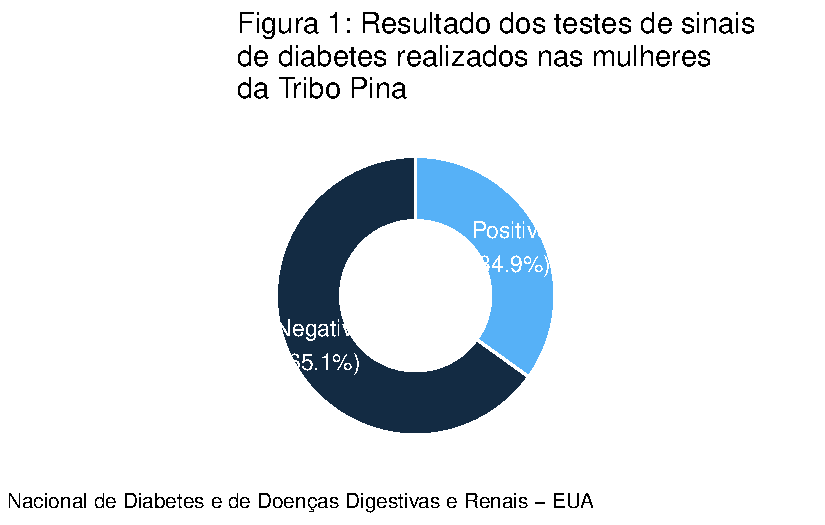
\includegraphics{relatorio_lab1_files/figure-pdf/unnamed-chunk-3-1.pdf}

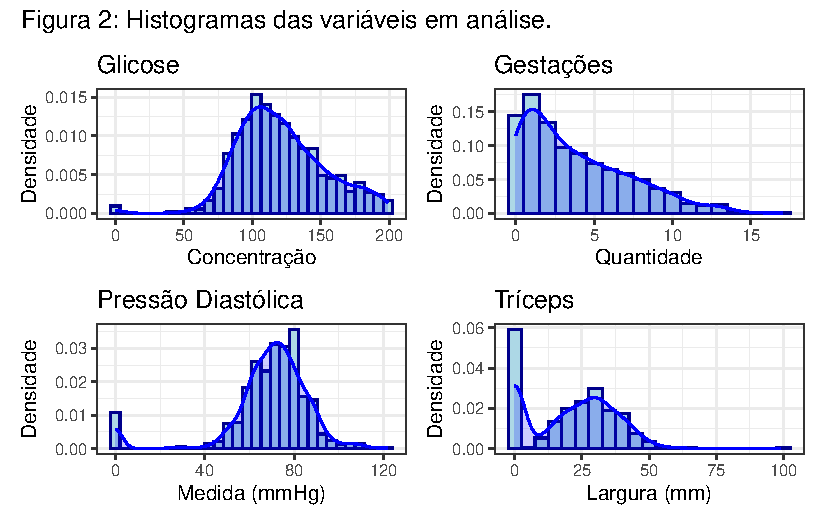
\includegraphics{relatorio_lab1_files/figure-pdf/unnamed-chunk-4-1.pdf}

\hypertarget{dados-tratados}{%
\subsection{Dados tratados}\label{dados-tratados}}

\begin{table}

\caption{Tabela 2: Medidas Resumo}
\centering
\begin{tabular}[t]{l|c|c|c|c|c|c|c|c}
\hline
  & Min & Q1 & Med & Média & Q3 & Max & Desvio Padrão & CV\\
\hline
\cellcolor{TRUE}{Glicose} & \cellcolor{TRUE}{56,00} & \cellcolor{TRUE}{99,00} & \cellcolor{TRUE}{119,00} & \cellcolor{TRUE}{122,63} & \cellcolor{TRUE}{143,00} & \cellcolor{TRUE}{198,00} & \cellcolor{TRUE}{30,86} & \cellcolor{TRUE}{0,25}\\
\hline
Idade & 21,00 & 23,00 & 27,00 & 30,86 & 36,00 & 81,00 & 10,20 & 0,33\\
\hline
\cellcolor{TRUE}{IMC} & \cellcolor{TRUE}{18,20} & \cellcolor{TRUE}{28,40} & \cellcolor{TRUE}{33,20} & \cellcolor{TRUE}{33,09} & \cellcolor{TRUE}{37,10} & \cellcolor{TRUE}{67,10} & \cellcolor{TRUE}{7,03} & \cellcolor{TRUE}{0,21}\\
\hline
Largura Triceps & 7,00 & 21,00 & 29,00 & 29,15 & 37,00 & 63,00 & 10,52 & 0,36\\
\hline
\cellcolor{TRUE}{N° de Gestações} & \cellcolor{TRUE}{0,00} & \cellcolor{TRUE}{1,00} & \cellcolor{TRUE}{2,00} & \cellcolor{TRUE}{3,30} & \cellcolor{TRUE}{5,00} & \cellcolor{TRUE}{17,00} & \cellcolor{TRUE}{3,21} & \cellcolor{TRUE}{0,97}\\
\hline
Nivel Diabético & 0,09 & 0,27 & 0,45 & 0,52 & 0,69 & 2,42 & 0,35 & 0,66\\
\hline
\cellcolor{TRUE}{Nível Insulina} & \cellcolor{TRUE}{14,00} & \cellcolor{TRUE}{76,50} & \cellcolor{TRUE}{125,50} & \cellcolor{TRUE}{156,06} & \cellcolor{TRUE}{190,00} & \cellcolor{TRUE}{846,00} & \cellcolor{TRUE}{118,84} & \cellcolor{TRUE}{0,76}\\
\hline
P. Diastólica & 24,00 & 62,00 & 70,00 & 70,66 & 78,00 & 110,00 & 12,50 & 0,18\\
\hline
\multicolumn{9}{l}{\rule{0pt}{1em}\textit{Note: }}\\
\multicolumn{9}{l}{\rule{0pt}{1em}Instituto Nacional de Diabetes e de Doenças Digestivas e Renais - EUA}\\
\end{tabular}
\end{table}

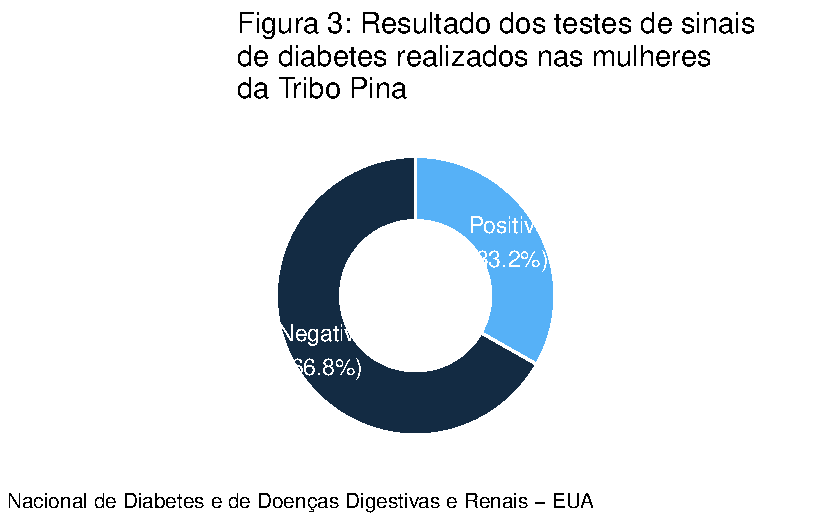
\includegraphics{relatorio_lab1_files/figure-pdf/unnamed-chunk-6-1.pdf}

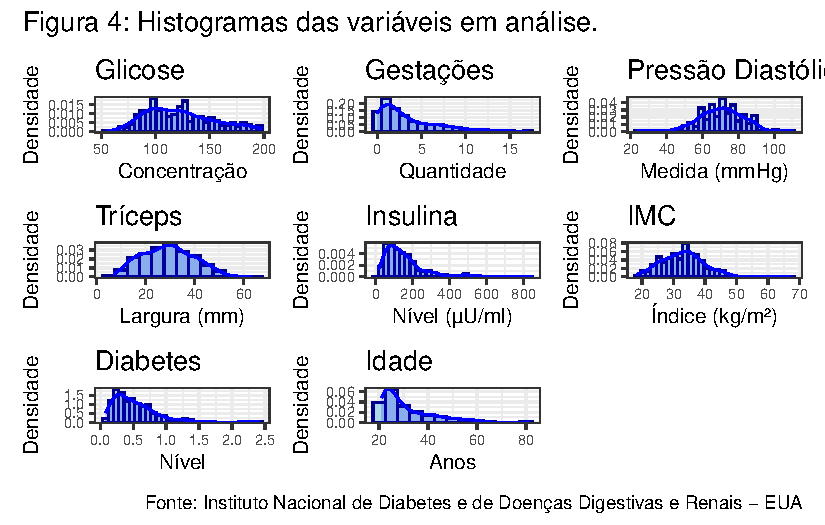
\includegraphics{relatorio_lab1_files/figure-pdf/unnamed-chunk-8-1.pdf}

\hypertarget{boxplot}{%
\subsection{Boxplot}\label{boxplot}}

\begin{Shaded}
\begin{Highlighting}[]
\DocumentationTok{\#\# Boxplot {-}{-}{-}{-}}
\NormalTok{b1 }\OtherTok{\textless{}{-}}\NormalTok{ dados}\SpecialCharTok{|\textgreater{}}
  \FunctionTok{filter}\NormalTok{(glucose}\SpecialCharTok{\textgreater{}}\DecValTok{0}\NormalTok{, diabetes}\SpecialCharTok{\textgreater{}}\DecValTok{0}\NormalTok{, diastolic}\SpecialCharTok{\textgreater{}}\DecValTok{0}\NormalTok{,}
\NormalTok{         triceps}\SpecialCharTok{\textgreater{}}\DecValTok{0}\NormalTok{, insulin}\SpecialCharTok{\textgreater{}}\DecValTok{0}\NormalTok{, bmi}\SpecialCharTok{\textgreater{}}\DecValTok{0}\NormalTok{)}\SpecialCharTok{|\textgreater{}}
  \FunctionTok{mutate}\NormalTok{(}
    \AttributeTok{test =} \FunctionTok{as\_factor}\NormalTok{(test),}
    \AttributeTok{test =} \FunctionTok{lvls\_revalue}\NormalTok{(test, }\FunctionTok{c}\NormalTok{(}\StringTok{"Negativo"}\NormalTok{, }\StringTok{"Positivo"}\NormalTok{))}
\NormalTok{  )}\SpecialCharTok{|\textgreater{}}
  \FunctionTok{ggplot}\NormalTok{(}\FunctionTok{aes}\NormalTok{(}\AttributeTok{x =}\NormalTok{ test, }\AttributeTok{y =}\NormalTok{ pregnant)) }\SpecialCharTok{+}
  \FunctionTok{geom\_boxplot}\NormalTok{(}\AttributeTok{col=}\StringTok{"darkblue"}\NormalTok{, }\AttributeTok{fill=}\StringTok{"skyblue"}\NormalTok{, }\AttributeTok{alpha =} \FloatTok{0.5}\NormalTok{)}\SpecialCharTok{+}
  \FunctionTok{labs}\NormalTok{(}
    \AttributeTok{title =} \StringTok{\textquotesingle{}N° de Gestações\textquotesingle{}}\NormalTok{,}
    \AttributeTok{x =} \StringTok{"Sinais de diabetes"}\NormalTok{,}
    \AttributeTok{y =} \StringTok{"Gestações"}
\NormalTok{  ) }\SpecialCharTok{+}
  \FunctionTok{scale\_y\_continuous}\NormalTok{(}
    \AttributeTok{labels =}\NormalTok{ scales}\SpecialCharTok{::}\FunctionTok{number\_format}\NormalTok{(}
      \AttributeTok{big.mark =} \StringTok{"."}\NormalTok{,}
      \AttributeTok{decimal.mark =} \StringTok{","}\NormalTok{))}\SpecialCharTok{+}
  \FunctionTok{theme\_bw}\NormalTok{()}
  
\NormalTok{b2 }\OtherTok{\textless{}{-}}\NormalTok{ dados}\SpecialCharTok{|\textgreater{}}
  \FunctionTok{filter}\NormalTok{(glucose}\SpecialCharTok{\textgreater{}}\DecValTok{0}\NormalTok{, diabetes}\SpecialCharTok{\textgreater{}}\DecValTok{0}\NormalTok{, diastolic}\SpecialCharTok{\textgreater{}}\DecValTok{0}\NormalTok{,}
\NormalTok{         triceps}\SpecialCharTok{\textgreater{}}\DecValTok{0}\NormalTok{, insulin}\SpecialCharTok{\textgreater{}}\DecValTok{0}\NormalTok{, bmi}\SpecialCharTok{\textgreater{}}\DecValTok{0}\NormalTok{)}\SpecialCharTok{|\textgreater{}}
  \FunctionTok{mutate}\NormalTok{(}
    \AttributeTok{test =} \FunctionTok{as\_factor}\NormalTok{(test),}
    \AttributeTok{test =} \FunctionTok{lvls\_revalue}\NormalTok{(test, }\FunctionTok{c}\NormalTok{(}\StringTok{"Negativo"}\NormalTok{, }\StringTok{"Positivo"}\NormalTok{))}
\NormalTok{  )}\SpecialCharTok{|\textgreater{}}
  \FunctionTok{ggplot}\NormalTok{(}\FunctionTok{aes}\NormalTok{(}\AttributeTok{x =}\NormalTok{ test, }\AttributeTok{y =}\NormalTok{ glucose)) }\SpecialCharTok{+}
  \FunctionTok{geom\_boxplot}\NormalTok{(}\AttributeTok{col=}\StringTok{"darkblue"}\NormalTok{, }\AttributeTok{fill=}\StringTok{"skyblue"}\NormalTok{, }\AttributeTok{alpha =} \FloatTok{0.5}\NormalTok{)}\SpecialCharTok{+}
  \FunctionTok{labs}\NormalTok{(}
    \AttributeTok{title =} \StringTok{\textquotesingle{}Nível de Glicose\textquotesingle{}}\NormalTok{,}
    \AttributeTok{x =} \StringTok{"Sinais de diabetes"}\NormalTok{,}
    \AttributeTok{y =} \StringTok{"Glicose"}
\NormalTok{  ) }\SpecialCharTok{+}
  \FunctionTok{scale\_y\_continuous}\NormalTok{(}
    \AttributeTok{labels =}\NormalTok{ scales}\SpecialCharTok{::}\FunctionTok{number\_format}\NormalTok{(}
      \AttributeTok{big.mark =} \StringTok{"."}\NormalTok{,}
      \AttributeTok{decimal.mark =} \StringTok{","}\NormalTok{))}\SpecialCharTok{+}
  \FunctionTok{theme\_bw}\NormalTok{()}

\NormalTok{b3 }\OtherTok{\textless{}{-}}\NormalTok{ dados}\SpecialCharTok{|\textgreater{}}
  \FunctionTok{filter}\NormalTok{(glucose}\SpecialCharTok{\textgreater{}}\DecValTok{0}\NormalTok{, diabetes}\SpecialCharTok{\textgreater{}}\DecValTok{0}\NormalTok{, diastolic}\SpecialCharTok{\textgreater{}}\DecValTok{0}\NormalTok{,}
\NormalTok{         triceps}\SpecialCharTok{\textgreater{}}\DecValTok{0}\NormalTok{, insulin}\SpecialCharTok{\textgreater{}}\DecValTok{0}\NormalTok{, bmi}\SpecialCharTok{\textgreater{}}\DecValTok{0}\NormalTok{)}\SpecialCharTok{|\textgreater{}}
  \FunctionTok{mutate}\NormalTok{(}
    \AttributeTok{test =} \FunctionTok{as\_factor}\NormalTok{(test),}
    \AttributeTok{test =} \FunctionTok{lvls\_revalue}\NormalTok{(test, }\FunctionTok{c}\NormalTok{(}\StringTok{"Negativo"}\NormalTok{, }\StringTok{"Positivo"}\NormalTok{))}
\NormalTok{  )}\SpecialCharTok{|\textgreater{}}
  \FunctionTok{ggplot}\NormalTok{(}\FunctionTok{aes}\NormalTok{(}\AttributeTok{x =}\NormalTok{ test, }\AttributeTok{y =}\NormalTok{ diastolic)) }\SpecialCharTok{+}
  \FunctionTok{geom\_boxplot}\NormalTok{(}\AttributeTok{col=}\StringTok{"darkblue"}\NormalTok{, }\AttributeTok{fill=}\StringTok{"skyblue"}\NormalTok{, }\AttributeTok{alpha =} \FloatTok{0.5}\NormalTok{)}\SpecialCharTok{+}
  \FunctionTok{labs}\NormalTok{(}
    \AttributeTok{title =} \StringTok{\textquotesingle{}Pressão Diastólica\textquotesingle{}}\NormalTok{,}
    \AttributeTok{x =} \StringTok{"Sinais de diabetes"}\NormalTok{,}
    \AttributeTok{y =} \StringTok{"Pressão Diastólica"}
\NormalTok{  ) }\SpecialCharTok{+}
  \FunctionTok{scale\_y\_continuous}\NormalTok{(}
    \AttributeTok{labels =}\NormalTok{ scales}\SpecialCharTok{::}\FunctionTok{number\_format}\NormalTok{(}
      \AttributeTok{big.mark =} \StringTok{"."}\NormalTok{,}
      \AttributeTok{decimal.mark =} \StringTok{","}\NormalTok{))}\SpecialCharTok{+}
  \FunctionTok{theme\_bw}\NormalTok{()}

\NormalTok{b4 }\OtherTok{\textless{}{-}}\NormalTok{ dados}\SpecialCharTok{|\textgreater{}}
  \FunctionTok{filter}\NormalTok{(glucose}\SpecialCharTok{\textgreater{}}\DecValTok{0}\NormalTok{, diabetes}\SpecialCharTok{\textgreater{}}\DecValTok{0}\NormalTok{, diastolic}\SpecialCharTok{\textgreater{}}\DecValTok{0}\NormalTok{,}
\NormalTok{         triceps}\SpecialCharTok{\textgreater{}}\DecValTok{0}\NormalTok{, insulin}\SpecialCharTok{\textgreater{}}\DecValTok{0}\NormalTok{, bmi}\SpecialCharTok{\textgreater{}}\DecValTok{0}\NormalTok{)}\SpecialCharTok{|\textgreater{}}
  \FunctionTok{mutate}\NormalTok{(}
    \AttributeTok{test =} \FunctionTok{as\_factor}\NormalTok{(test),}
    \AttributeTok{test =} \FunctionTok{lvls\_revalue}\NormalTok{(test, }\FunctionTok{c}\NormalTok{(}\StringTok{"Negativo"}\NormalTok{, }\StringTok{"Positivo"}\NormalTok{))}
\NormalTok{  )}\SpecialCharTok{|\textgreater{}}
  \FunctionTok{ggplot}\NormalTok{(}\FunctionTok{aes}\NormalTok{(}\AttributeTok{x =}\NormalTok{ test, }\AttributeTok{y =}\NormalTok{ insulin)) }\SpecialCharTok{+}
  \FunctionTok{geom\_boxplot}\NormalTok{(}\AttributeTok{col=}\StringTok{"darkblue"}\NormalTok{, }\AttributeTok{fill=}\StringTok{"skyblue"}\NormalTok{, }\AttributeTok{alpha =} \FloatTok{0.5}\NormalTok{)}\SpecialCharTok{+}
  \FunctionTok{labs}\NormalTok{(}
    \AttributeTok{title =} \StringTok{\textquotesingle{}Nível de Insulina\textquotesingle{}}\NormalTok{,}
    \AttributeTok{x =} \StringTok{"Sinais de diabetes"}\NormalTok{,}
    \AttributeTok{y =} \StringTok{"Nível de Insulina"}
\NormalTok{  ) }\SpecialCharTok{+}
  \FunctionTok{scale\_y\_continuous}\NormalTok{(}
    \AttributeTok{labels =}\NormalTok{ scales}\SpecialCharTok{::}\FunctionTok{number\_format}\NormalTok{(}
      \AttributeTok{big.mark =} \StringTok{"."}\NormalTok{,}
      \AttributeTok{decimal.mark =} \StringTok{","}\NormalTok{))}\SpecialCharTok{+}
  \FunctionTok{theme\_bw}\NormalTok{()}

\NormalTok{b5 }\OtherTok{\textless{}{-}}\NormalTok{ dados}\SpecialCharTok{|\textgreater{}}
  \FunctionTok{filter}\NormalTok{(glucose}\SpecialCharTok{\textgreater{}}\DecValTok{0}\NormalTok{, diabetes}\SpecialCharTok{\textgreater{}}\DecValTok{0}\NormalTok{, diastolic}\SpecialCharTok{\textgreater{}}\DecValTok{0}\NormalTok{,}
\NormalTok{         triceps}\SpecialCharTok{\textgreater{}}\DecValTok{0}\NormalTok{, insulin}\SpecialCharTok{\textgreater{}}\DecValTok{0}\NormalTok{, bmi}\SpecialCharTok{\textgreater{}}\DecValTok{0}\NormalTok{)}\SpecialCharTok{|\textgreater{}}
  \FunctionTok{mutate}\NormalTok{(}
    \AttributeTok{test =} \FunctionTok{as\_factor}\NormalTok{(test),}
    \AttributeTok{test =} \FunctionTok{lvls\_revalue}\NormalTok{(test, }\FunctionTok{c}\NormalTok{(}\StringTok{"Negativo"}\NormalTok{, }\StringTok{"Positivo"}\NormalTok{))}
\NormalTok{  )}\SpecialCharTok{|\textgreater{}}
  \FunctionTok{ggplot}\NormalTok{(}\FunctionTok{aes}\NormalTok{(}\AttributeTok{x =}\NormalTok{ test, }\AttributeTok{y =}\NormalTok{ bmi)) }\SpecialCharTok{+}
  \FunctionTok{geom\_boxplot}\NormalTok{(}\AttributeTok{col=}\StringTok{"darkblue"}\NormalTok{, }\AttributeTok{fill=}\StringTok{"skyblue"}\NormalTok{, }\AttributeTok{alpha =} \FloatTok{0.5}\NormalTok{)}\SpecialCharTok{+}
  \FunctionTok{labs}\NormalTok{(}
    \AttributeTok{title =} \StringTok{\textquotesingle{}IMC\textquotesingle{}}\NormalTok{,}
    \AttributeTok{x =} \StringTok{"Sinais de diabetes"}\NormalTok{,}
    \AttributeTok{y =} \StringTok{"IMC"}
\NormalTok{  ) }\SpecialCharTok{+}
  \FunctionTok{scale\_y\_continuous}\NormalTok{(}
    \AttributeTok{labels =}\NormalTok{ scales}\SpecialCharTok{::}\FunctionTok{number\_format}\NormalTok{(}
      \AttributeTok{big.mark =} \StringTok{"."}\NormalTok{,}
      \AttributeTok{decimal.mark =} \StringTok{","}\NormalTok{))}\SpecialCharTok{+}
  \FunctionTok{theme\_bw}\NormalTok{()}

\NormalTok{b6 }\OtherTok{\textless{}{-}}\NormalTok{ dados}\SpecialCharTok{|\textgreater{}}
  \FunctionTok{filter}\NormalTok{(glucose}\SpecialCharTok{\textgreater{}}\DecValTok{0}\NormalTok{, diabetes}\SpecialCharTok{\textgreater{}}\DecValTok{0}\NormalTok{, diastolic}\SpecialCharTok{\textgreater{}}\DecValTok{0}\NormalTok{,}
\NormalTok{         triceps}\SpecialCharTok{\textgreater{}}\DecValTok{0}\NormalTok{, insulin}\SpecialCharTok{\textgreater{}}\DecValTok{0}\NormalTok{, bmi}\SpecialCharTok{\textgreater{}}\DecValTok{0}\NormalTok{)}\SpecialCharTok{|\textgreater{}}
  \FunctionTok{mutate}\NormalTok{(}
    \AttributeTok{test =} \FunctionTok{as\_factor}\NormalTok{(test),}
    \AttributeTok{test =} \FunctionTok{lvls\_revalue}\NormalTok{(test, }\FunctionTok{c}\NormalTok{(}\StringTok{"Negativo"}\NormalTok{, }\StringTok{"Positivo"}\NormalTok{))}
\NormalTok{  )}\SpecialCharTok{|\textgreater{}}
  \FunctionTok{ggplot}\NormalTok{(}\FunctionTok{aes}\NormalTok{(}\AttributeTok{x =}\NormalTok{ test, }\AttributeTok{y =}\NormalTok{ triceps)) }\SpecialCharTok{+}
  \FunctionTok{geom\_boxplot}\NormalTok{(}\AttributeTok{col=}\StringTok{"darkblue"}\NormalTok{, }\AttributeTok{fill=}\StringTok{"skyblue"}\NormalTok{, }\AttributeTok{alpha =} \FloatTok{0.5}\NormalTok{)}\SpecialCharTok{+}
  \FunctionTok{labs}\NormalTok{(}
    \AttributeTok{title =} \StringTok{\textquotesingle{}Largura do Tríceps\textquotesingle{}}\NormalTok{,}
    \AttributeTok{x =} \StringTok{"Sinais de diabetes"}\NormalTok{,}
    \AttributeTok{y =} \StringTok{"Tríceps"}
\NormalTok{  ) }\SpecialCharTok{+}
  \FunctionTok{scale\_y\_continuous}\NormalTok{(}
    \AttributeTok{labels =}\NormalTok{ scales}\SpecialCharTok{::}\FunctionTok{number\_format}\NormalTok{(}
      \AttributeTok{big.mark =} \StringTok{"."}\NormalTok{,}
      \AttributeTok{decimal.mark =} \StringTok{","}\NormalTok{))}\SpecialCharTok{+}
  \FunctionTok{theme\_bw}\NormalTok{()}

\NormalTok{b1}\SpecialCharTok{+}\NormalTok{b2}\SpecialCharTok{+}\NormalTok{b3}\SpecialCharTok{+}\NormalTok{b4}\SpecialCharTok{+}\NormalTok{b5}\SpecialCharTok{+}\NormalTok{b6 }\SpecialCharTok{+} 
  \FunctionTok{plot\_layout}\NormalTok{(}\AttributeTok{nrow =} \DecValTok{2}\NormalTok{, }\AttributeTok{ncol =} \DecValTok{3}\NormalTok{) }\SpecialCharTok{+} 
  \FunctionTok{plot\_annotation}\NormalTok{(}
    \AttributeTok{title =} \StringTok{"Figura : "}\NormalTok{,}
    \AttributeTok{caption =} \StringTok{"Fonte: Instituto Nacional de Diabetes e de Doenças Digestivas e Renais {-} EUA"}
    \CommentTok{\# tag\_levels = c("A", "1"), tag\_prefix = "Sub Fig. ", tag\_sep = ".",}
    \CommentTok{\# tag\_levels = "A",}
    \CommentTok{\# tag\_suffix = ":"}
\NormalTok{  ) }\SpecialCharTok{\&} \FunctionTok{theme\_bw}\NormalTok{(}\AttributeTok{base\_size =} \DecValTok{10}\NormalTok{) }\SpecialCharTok{\&}
  \FunctionTok{theme}\NormalTok{(}
    \AttributeTok{plot.tag.position =} \FunctionTok{c}\NormalTok{(}\DecValTok{0}\NormalTok{, }\DecValTok{1}\NormalTok{),}
    \AttributeTok{plot.tag =} \FunctionTok{element\_text}\NormalTok{(}\AttributeTok{size =} \DecValTok{12}\NormalTok{, }\AttributeTok{hjust =} \DecValTok{0}\NormalTok{, }\AttributeTok{vjust =} \DecValTok{0}\NormalTok{)}
\NormalTok{  )}
\end{Highlighting}
\end{Shaded}

\begin{figure}[H]

{\centering 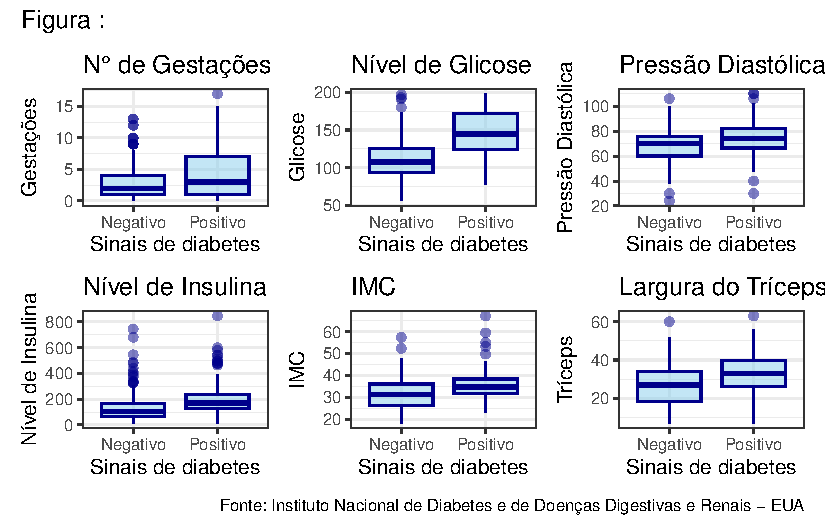
\includegraphics{relatorio_lab1_files/figure-pdf/unnamed-chunk-9-1.pdf}

}

\end{figure}



\end{document}
